\documentclass{standalone}
\newcommand{\repeater}[3]{%
 \node ({#1}) at ({#2}) {%
  \begin{tikzpicture}%
   \draw [black,thick] (-.25,0) -- (0,0.5) -- (0.25,0) -- (-0.25,0);%
   \draw [black,thick,domain=-45:225] plot ({0.2*cos(\x)}, {0.5+0.2*sin(\x)});%
   \draw [black,thick,domain=-45:225] plot ({0.4*cos(\x)}, {0.5+0.4*sin(\x)});%
   \node (xxx) at (0,-.2) {{#3}};%
  \end{tikzpicture}%
 } %
}

\newcommand{\activerepeater}[3]{%
 \node ({#1}) at ({#2}) {%
  \begin{tikzpicture}%
   \draw [black,thick] (-.25,0) -- (0,0.5) -- (0.25,0) -- (-0.25,0);%
   \draw [red,thick,domain=-45:225] plot ({0.2*cos(\x)}, {0.5+0.2*sin(\x)});%
   \draw [red,thick,domain=-45:225] plot ({0.4*cos(\x)}, {0.5+0.4*sin(\x)});%
   \node (xxx) at (0,-.2) {{#3}};%
  \end{tikzpicture}%
 } %
}


\newcommand{\user}[3]{%
 \node ({#1}) at ({#2}) {%
  \begin{tikzpicture}%
   \draw [black,fill=black] (-.25,0) -- (0,0.5) -- (0.25,0) -- (-0.25,0);%
   \draw [black,fill=black] (0,.5) circle (.2); %
   \node (xxx) [text width=0.6cm, align=center] at (-.35cm,-.4) {{#3}};%
  \end{tikzpicture}%
 } %
}

\newcommand{\activeuser}[3]{%
 \node ({#1}) at ({#2}) {%
  \begin{tikzpicture}%
   \draw [red,fill=red] (-.25,0) -- (0,0.5) -- (0.25,0) -- (-0.25,0);%
   \draw [red,fill=red] (0,.5) circle (.2); %
   \node (xxx) [text width=0.6cm, align=center] at (-.35cm,-.4) {{#3}};%
  \end{tikzpicture}%
 } %
}

\begin{document}
  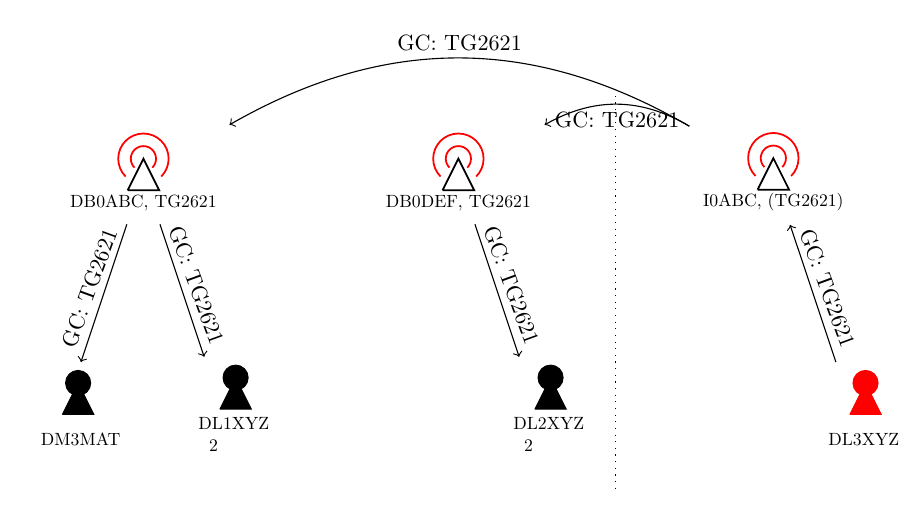
\begin{tikzpicture}[every node/.style={scale=.8}]
   \user{u1}{ 0,0}{DM3MAT};
   \user{u2}{ 2,0}{DL1XYZ 2};	
   \user{u3}{ 6,0}{DL2XYZ 2};	
   \draw[dotted] (7,4) -- (7,-1);
   \activeuser{u4}{10,0}{DL3XYZ};
   \activerepeater{R1}{1,3}{DB0ABC, TG2621};
   \activerepeater{R2}{5,3}{DB0DEF, TG2621};
   \activerepeater{R3}{9,3}{I0ABC, (TG2621)};
   \path[->] (u4) edge node[above,rotate=-70]{GC: TG2621} (R3);
   \path[->] (R1) edge node[above,rotate=70]{GC: TG2621} (u1);
   \path[->] (R1) edge node[above,rotate=-70]{GC: TG2621} (u2);
   \path[->] (R2) edge node[above,rotate=-70]{GC: TG2621} (u3);
   \path[->] (R3) edge[bend right] node[below]{GC: TG2621} (R2);
   \path[->] (R3) edge[bend right] node[above]{GC: TG2621} (R1);
  \end{tikzpicture}
\end{document}
